\documentclass[border=6pt]{standalone}
\usepackage[T1]{fontenc}
\usepackage{courier}
\usepackage[scaled=0.95]{helvet}
\renewcommand{\familydefault}{\sfdefault}
\usepackage{sfmath}
\usepackage[version=4]{mhchem}
\usepackage{tikz}
\usepackage{pgfplots}
\pgfplotsset{compat=newest}
\usetikzlibrary{arrows.meta,positioning,calc,fit,backgrounds,shapes.geometric,decorations.pathreplacing,patterns}
\definecolor{ink}{HTML}{17233A}
\definecolor{inksoft}{HTML}{44506A}
\definecolor{teal}{HTML}{0E6B6B}
\definecolor{tealsoft}{HTML}{E5F0EF}
\definecolor{amber}{HTML}{B26B12}
\definecolor{ambersoft}{HTML}{FBF0DF}
\definecolor{blue}{HTML}{2F6690}
\definecolor{bluesoft}{HTML}{E3ECF4}
\definecolor{plum}{HTML}{7A4D8C}
\definecolor{plumsoft}{HTML}{EFE7F3}
\definecolor{greyc}{HTML}{8A94A3}
\definecolor{linec}{HTML}{D3DCE1}
\definecolor{oxy}{HTML}{C0392B}
\definecolor{carb}{HTML}{3B4252}
\definecolor{hyd}{HTML}{E6E9EE}
\definecolor{nit}{HTML}{2F6690}
\tikzset{
  every picture/.style={line cap=round,line join=round},
  lab/.style={font=\small, text=inksoft},
  >={Stealth[length=7pt]},
}
\pgfplotsset{
  every axis/.append style={axis line style={inksoft}, tick style={inksoft}, tick label style={font=\footnotesize, text=inksoft}, label style={font=\small, text=ink}},
}
% fragment tile: \frag{node name}{position}{colour}{content}
\newcommand{\frag}[4]{\node[draw=#3, fill=#3!12, line width=1.4pt, rounded corners=6pt, minimum width=1.25cm, minimum height=1.05cm, text=#3, font=\bfseries] (#1) at (#2) {#4};}
\newcommand{\ring}{\tikz[baseline=-0.6ex]{\draw[line width=1.1pt] (0:0.3)--(60:0.3)--(120:0.3)--(180:0.3)--(240:0.3)--(300:0.3)--cycle; \draw[line width=0.8pt] (0,0) circle (0.16);}}
\newcommand{\bond}[2]{\draw[ink, line width=2.2pt] (#1) -- (#2);}

\begin{document}
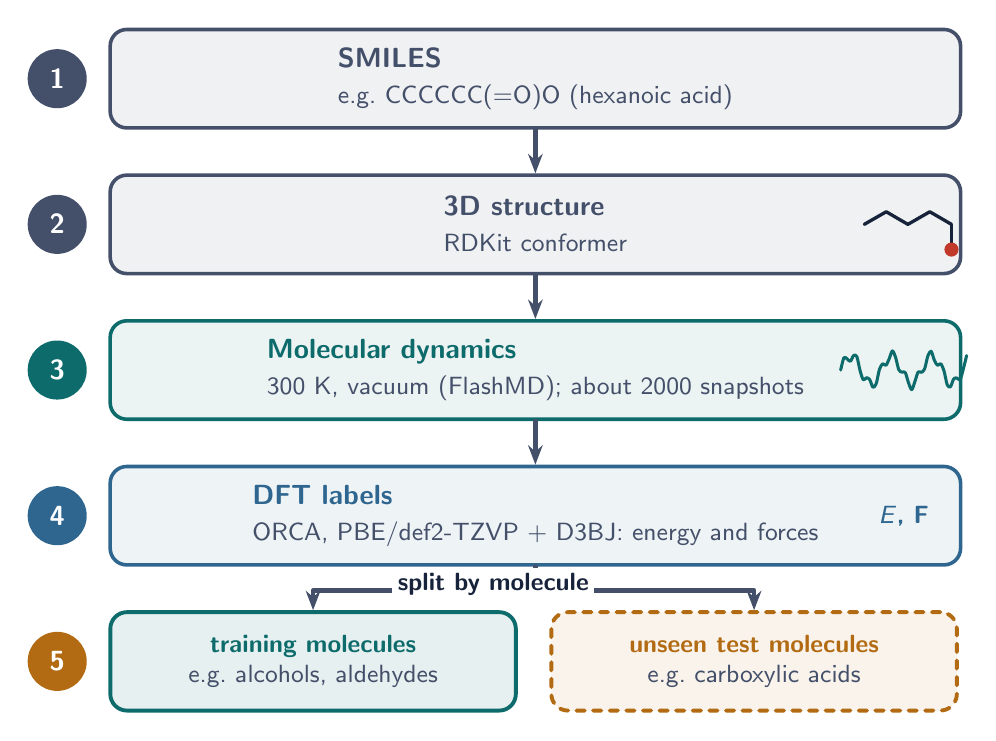
\begin{tikzpicture}[box/.style={draw=#1, line width=1.3pt, rounded corners=6pt, fill=#1!8, minimum width=10.8cm, minimum height=1.25cm, align=left, inner xsep=10pt}]
\node[box=inksoft, anchor=west] (s0) at (0,0.00) {\textbf{\textcolor{inksoft}{SMILES}}\\[1pt]{\small\textcolor{inksoft}{e.g.\ CCCCCC(=O)O (hexanoic acid)}}};
\node[circle, fill=inksoft, text=white, font=\bfseries, minimum size=0.75cm] at (-0.65,0.00) {1};
\node[box=inksoft, anchor=west] (s1) at (0,-1.85) {\textbf{\textcolor{inksoft}{3D structure}}\\[1pt]{\small\textcolor{inksoft}{RDKit conformer}}};
\node[circle, fill=inksoft, text=white, font=\bfseries, minimum size=0.75cm] at (-0.65,-1.85) {2};
\draw[->, inksoft, line width=1.6pt] (s0.south) -- (s1.north);
\node[box=teal, anchor=west] (s2) at (0,-3.70) {\textbf{\textcolor{teal}{Molecular dynamics}}\\[1pt]{\small\textcolor{inksoft}{300 K, vacuum (FlashMD); about 2000 snapshots}}};
\node[circle, fill=teal, text=white, font=\bfseries, minimum size=0.75cm] at (-0.65,-3.70) {3};
\draw[->, inksoft, line width=1.6pt] (s1.south) -- (s2.north);
\node[box=blue, anchor=west] (s3) at (0,-5.55) {\textbf{\textcolor{blue}{DFT labels}}\\[1pt]{\small\textcolor{inksoft}{ORCA, PBE/def2-TZVP + D3BJ: energy and forces}}};
\node[circle, fill=blue, text=white, font=\bfseries, minimum size=0.75cm] at (-0.65,-5.55) {4};
\draw[->, inksoft, line width=1.6pt] (s2.south) -- (s3.north);
\begin{scope}[shift={(9.6,-1.85)}, scale=0.32] \draw[ink, line width=1.2pt] (0,0)--(0.87,0.5)--(1.73,0)--(2.6,0.5)--(3.46,0); \draw[ink, line width=1.2pt] (3.46,0)--(3.46,-0.9); \fill[oxy] (3.46,-1.0) circle (0.28); \end{scope}
\begin{scope}[shift={(9.3,-3.70)}] \draw[teal, line width=1.1pt] plot[smooth, domain=0:1.6, samples=40] (\x,{0.18*sin(\x*700)+0.07*sin(\x*2300)}); \end{scope}
\node[font=\small\bfseries, text=blue] at (10.1,-5.55) {$E$, $\mathbf{F}$};
\node[draw=teal, line width=1.4pt, rounded corners=6pt, fill=teal!10, minimum width=5.15cm, minimum height=1.25cm, align=center, anchor=west, font=\small] (tr) at (0,-7.40) {\textbf{\textcolor{teal}{training molecules}}\\\textcolor{inksoft}{e.g.\ alcohols, aldehydes}};
\node[draw=amber, line width=1.4pt, dashed, rounded corners=6pt, fill=amber!8, minimum width=5.15cm, minimum height=1.25cm, align=center, anchor=east, font=\small] (te) at (10.8,-7.40) {\textbf{\textcolor{amber}{unseen test molecules}}\\\textcolor{inksoft}{e.g.\ carboxylic acids}};
\node[circle, fill=amber, text=white, font=\bfseries, minimum size=0.75cm] at (-0.65,-7.40) {5};
\draw[->, inksoft, line width=1.6pt] (s3.south) -- ++(0,-0.3) -| (tr.north);
\draw[->, inksoft, line width=1.6pt] (s3.south) -- ++(0,-0.3) -| (te.north);
\node[font=\small\bfseries, text=ink, anchor=west, fill=white, inner sep=2pt] at (3.6,-6.42) {split by molecule};
\end{tikzpicture}
\end{document}
